
\documentclass[12 pt]{article}
%\usepackage[letterpaper,hmargin=1in,vmargin=1.5in]{geometry}
\usepackage{indentfirst,mathrsfs}
\usepackage{amsfonts}
\usepackage{amsmath,amsthm,amssymb}
\usepackage{enumitem}
\usepackage[colorlinks,linkcolor=black,
            pdftitle={title},
              pdfauthor={author},
              pdfkeywords={}]{hyperref}
\usepackage{tikz}              
\renewcommand{\baselinestretch}{1.2}
\usetikzlibrary{matrix}

\setlength{\oddsidemargin}{0.1in} \setlength{\textwidth}{6.0in}
\setlength{\topmargin}{-0.25in} \setlength{\textheight}{8.7in}

\newtheorem{theorem}{Theorem}
\newtheorem{corollary}{Corollary}
\newtheorem{definition}{Definition}
\newtheorem{Example}{Example}
\newtheorem{proposition}{Proposition}
\newtheorem{construction}{Construction}
\newtheorem{remark}{Remark}
\newtheorem{exm}{Example}
\newtheorem{lemma}{Lemma}
\def\E{{\mathbb E}}
\def\F{{\mathbb F}}

\newcommand{\tr}{\operatorname{tr}_1^n}

\begin{document}




\begin{theorem}
    Let $ F(x) = x^{q^2+q+1} \in\F_{q^4}[x] $, where $ q = 2^k $. Then for any nonzero $ u,v $, the second-order 
  \end{theorem}
  
  \begin{proof}
    Note that for $ a\ne 0 $ and $ \forall u,v\in\F_{2^n} $ with $ v\ne 0 $, we have
    \begin{align*}
      W_{D_aF}(u,v)&=\sum_{x\in\F_{2^n}}(-1)^{\tr(v(D_aF(x))+ux)}\\
                   &=\sum_{x\in\F_{2^n}}(-1)^{\tr(v(F(x)+F(x+a))+ux)}\\
                  %  &=\sum_{x\in\F_{2^n}}(-1)^{\tr(v(x^{q^2+q+1}+(x+a)^{q^2+q+1})+ux)}\\
                   &=\sum_{x\in\F_{2^n}}(-1)^{\tr\left(v\left(x^{d}+(x+a)^{d}\right)+ux\right)}\\
                   &=\sum_{x\in\F_{2^n}}(-1)^{\tr\left(\left(\left(v^{\frac{1}{d}}x\right)^{d}+\left(v^{\frac{1}{d}}x+v^{\frac{1}{d}}a\right)^{d}\right)+ux\right)}\\
                   &=\sum_{x\in\F_{2^n}}(-1)^{\tr\left(\left(\left(v^{\frac{1}{d}}x\right)^{d}+\left(v^{\frac{1}{d}}x+v^{\frac{1}{d}}a\right)^{d}\right)+uv^{-\frac{1}{d}}v^{\frac{1}{d}}x\right)}\\
                   &=\sum_{x^{\prime}\in\F_{2^n}}(-1)^{\tr\left(\left(\left(x^{\prime}\right)^{d}+\left(x^{\prime}+v^{\frac{1}{d}}a\right)^{d}\right)+uv^{-\frac{1}{d}}x^{\prime}\right)}\\
                   &=W_{D_{a^{\prime}}F}\left(uv^{-\frac{1}{d}},1\right)
    \end{align*}
    where $ x^{\prime}=v^{\frac{1}{d}}x $ and $ a^{\prime}=v^{\frac{1}{d}}a $.
    Then once $ W_{D_aF}(u,1) $ is known for all $ a,u\in\F_{2^n} $, $ W_{D_aF}(u,v) $ will also be determined.
  
    Note that we have $ \deg(D_aF)=2 $ since $ \deg(F) = 3 $, i.e. $ D_aF(x) $ is a quadratic function.
    And the Walsh spectrum of a quadratic Boolean function is completely characterized by the  dimension 
    of the kernel of the bilinear form associated to it.  
    
    So we consider the bilinear form $ \mathcal{B}(x,y) $ associated with $ \tr\left(D_aF(x)\right) $, 
    and the function $ \mathcal{B}(x,y) $ becomes
    \begin{align*}
      \mathcal{B}(x,y)=& \tr\left(D_aF(0)\right)+\tr\left(D_aF(x)\right)+\tr\left(D_aF(y)\right)+\tr\left( D_aF(x+y) \right)\\
                      =& \tr\left(a^d\right)+\tr\left(x^d+(x+a)^d\right)+\tr\left(y^d+(y+a)^d\right)+\tr\left((x+y)^d+(x+y+a)^d\right)\\
                      =& \tr\left( a^qx^{q^2+1}+a^{q^2}x^{q+1}+ax^{q^2+q}+a^qy^{q^2+1}+a^{q^2}y^{q+1}+ay^{q^2+q}+a^q(x+y)^{q^2+1}\right.\\
                       &\left.+a^{q^2}(x+y)^{q+1}+a(x+y)^{q^2+q} \right)\\
                      =& \tr\left( a^q\left( x^{q^2}y+xy^{q^2} \right)+ a^{q^2}\left( x^qy+xy^q \right)+ a\left( x^{q^2}y^q+x^qy^{q^2} \right) \right)\\
                      =& \tr\left(y\widetilde{f}(x)^q\right).
    \end{align*}
    where 
    $ \widetilde{f}(x)=\left( a^{q}+a \right)x^{q^2}+\left( a^{q^2}+a \right)x^{q }+\left( a^{q }+a^{q^2} \right)x $
    and the kernel of $ \mathcal{B}(x,y) $ is equal to $ \mathcal{E}=\left\{ x\in\F_{2^n}\middle|\widetilde{f}(x)=0 \right\} $. 
  
    When the coefficient of $ x^{q^2} $ in $ \widetilde{f}(x) $ is zero, 
    we have $ a^q+a=0 $, i.e. $ a\in\F_q $, resulting in the coefficients of $ x^q $ and $ x $ both are $ 0 $, 
    which means that the kernel of $ \mathcal{B}(x,y) $ is $ \F_{2^n} $ for $ a\in\F_q $, 
    that is, the dimension of the kernel is $ n $.
  
    When $ a^q+a\ne 0 $, i.e. $ a\in\F_{2^n}\setminus\F_q $, 
    $ \widetilde{f}(x) $ is a linearized polynomial and we can transform it into 
    \begin{align*}
    \widetilde{f}(x)&=\left( a^{q}+a \right)x^{q^2}+\left( a^{q^2}+a \right)x^{q }+\left( a^{q }+a^{q^2} \right)x \\
                    &=\left( a^{q}+a \right)x^{q^2}+\left( a^q+a^{q^2}+a^q+a \right)x^{q }+\left( a^{q }+a^{q^2} \right)x \\
                    &=\left( a^{q}+a \right)\left( x^{q^2}+x^q \right)+\left( a^{q }+a^{q^2} \right)\left( x^q+x \right) \\
                    &=\left( a^{q}+a \right)\left( x^{q}+x \right)^q+\left( a+a^{q} \right)^q\left( x^q+x \right). 
    \end{align*}
    Note that $ a^q+a\ne 0 $, then $ \widetilde{f}(x)=0 $ implies that $ \left( x^{q}+x \right)^q+\left( a+a^{q} \right)^{q-1}\left( x^q+x \right)=0 $. Clearly all elements of $ \F_q $ are solutions of $ \widetilde{f}(x)=0 $, meanwhile, for $ x\in\F_{q^4}\setminus\F_q $, $ \widetilde{f}(x)=0 $ can get 
    \[\left( a+a^{q} \right)\left( x^q+x \right)\left( \left( x^q+x \right)^{q-1}+\left( a+a^q \right)^{q-1} \right)=0,\]
    implying that 
    \[\left( \frac{x^q+x}{a^q+a}  \right)^{q-1}=1.\]
    In other words, $ x\in\F_{q^4}\setminus\F_q $ is a solution of $ \widetilde{f}(x)=0 $ 
    if and only if $ \frac{x^q+x}{a^q+a}\in\F_q^* $. 
    Therefore assume $ \theta = \frac{x^q+x}{a^q+a}\in\F_q^* $, then we have $ x^q+x+\theta(a^q+a)=x^q+x+(\theta a)^q+\theta a=(x+\theta a)^q+(x+\theta a)=0 $, 
    which is equivalent to $ x+\theta a\in\F_q $. Thus we have $ x\in \theta a+\F_q $ 
    and the number of solutions $ x\in\F_{q^4}\setminus\F_q $ of $ \widetilde{f}(x)=0 $ is $ q(q-1) $ for $ a\in\F_{q^4}\setminus\F_q $.
    
    So the number of solutions of $ \widetilde{f}(x)=0 $ is $ q^4 $ 
    and $ q+q(q-1)=q^2 $ for $ a\in\F_q $ and  $ a\in\F_{q^4}\setminus\F_q $, respectively. 
    Thus,  
    \begin{align*}
      \dim_{\F_2}\mathcal{E}=\begin{cases}
        2k,&\text{~if~}a\in\F_{q^4}\setminus\F_q\\
        4k,&\text{~if~}a\in\F_q.\\
      \end{cases}
    \end{align*}
    Therefore, we have 
    
    \begin{equation*}
      \max_{u\in\F_{q^4}}\left\lvert W_{D_aF}(u,1)\right\rvert=\begin{cases}
        2^{3k},&\text{~if~}a\in\F_{q^4}\setminus\F_q\\
        2^{4k},&\text{~if~}a\in\F_{q}
      \end{cases}
    \end{equation*}
  \end{proof}

    \begin{theorem}[name of the theorem]
      Let $ F(x) = x^{2^{2i}-2^i+1}\in\F_{2^n}[x] $, where $ \gcd(i,n) = 1 $. Then for any $ \gamma,\eta,\omega $ we have 
      \[\mathcal{N}_F(\gamma,\eta,\omega)=\#\left\{ x\in\F_{2^n}:F(x)+F(x+\gamma)+F(x+\eta)+F(x+\gamma+\eta) = \omega \right\}\] 
      and the distribution of $ \mathcal{N}_F(\gamma,\eta,\omega) $ is 

    \end{theorem}
    Let $ d=2^{2i}-2^i+1=2^{i+i-1}+2^{i+i-2}+\cdots+2^i+1 $, note that the exponents of $ 2 $ are all distinct and we assume 
    a set $ D $ associated with $ d $ such that 
    \[D=\left\{ 0,i,i+1,\dots,i-2,i-1 \right\},\]
    then we can partition $ D $ into two disjoint sets $ J,K $ such that $ J\cap K=\emptyset $ and $ J\cup K=D $.
    Therefore we can rewrite $ (x+\gamma)^d $ as 
    \[ (x+\gamma)^d=\sum_{\substack{J\cap K=\emptyset\\J\cup K=D}}x^J\gamma^K, \]
    where we denote $ \prod_{j\in J}x^j $ by $ x^J $.
    \begin{proof}[To Be Conituned]
      We calculate the equation 
      \[F(x)+F(x+\gamma)+F(x+\eta)+F(x+\gamma+\eta) = \omega.\]
      After calculation we have 
      \[\sum_{\substack{J\cap K=\emptyset\\J\cup K=D\\1\le|J|\le i-1}}y^J\left[ \left( 1+\theta \right)^K+1+ \theta^K \right] = \omega^{\prime},\]
      where $ \theta=\frac{b}{a} $, $ y=\frac{x}{a} $ and $ \omega^{\prime}=\omega+cons $ with $ cons $ is the function of $ \gamma,\eta $ and we can 
      omit it since $ \omega $ ranges over $ \F_{2^n} $.

      For $ i=3 $, we 
    \end{proof}
      Let $ \mu_d $ be the $ d $-th roots of unity and $ q=2^{2m} $ with $ d\mid(q-1) $, where 
      $ d $ and $ m $ are positive integers. The unit circle of $ \F_q $ is defined by 
      \[\mu_{2^m+1}=\left\{ x\in\F_{q}:x^{2^m+1}=x\overline{x}=1 \right\}.\]
    \begin{theorem}[permutation polynomials like P.L. Sharma]
      The polynomial $ f(x)=x^bh(x^{2^m-1}) $ is a permutation polynomial over $ \F_{q} $, 
      where $ h(x)=1+x^a+x^b $, $ b=2^i+2^j,a=2^j $ and $ i>j $ with satisfying the system 
      \begin{equation}
        \left\{ 
        \begin{aligned}
          &\gcd(2^m+1,2^i-2^j-1)=1\\
          &\gcd(m,i-j)=\gcd(2m,i-j)=\gcd(m,2(i-j))\\
        \end{aligned}\right.
      \end{equation}
    \end{theorem}

    We will use Lemma below to prove the theorem.
    \begin{lemma}\label{Lm:permutation_twocondition}
      Let $ d,r>0 $ with $ d\mid(q-1) $ and $ h(x)\in\F_q[x] $. Then $ f(x)=x^rh(x^{\frac{q-1}{d}}) $ permute $ \F_q $ iff the following two conditions hold:
      \begin{enumerate}[label=(\arabic{*})]
        \item $ \gcd(r,(q-1)/d)=1 $,
        \item $ x^rh(x)^{(q-1)/{d}} $ permutes $ \mu_d $.
      \end{enumerate}
    \end{lemma}

    \begin{proof}[Proof of Theorem]
      The polynomial $ f(x) $ can be written as $ f(x)=x^b h\left(x^{2^m-1}\right)$, where $h(x)=1+x^a+x^b \in \F_{2^{2m}}[x]$. 
      Note that  
      \[\gcd(b,(q-1)/d)=\gcd(2^i+2^j,2^m-1)=\gcd(2^{i-j}+1,2^m-1)=1\]
      since $ \gcd(i-j,m)=\gcd(2(i-j),m) $, and then $ f(x) $ permutes $ \F_q $ iff the polynomial $ g(x)=x^bh(x)^{2^m-1} $ 
      permutes $ \mu_{2^m+1} $ by Lemma \ref{Lm:permutation_twocondition}.
      
      The inexistence of roots of polynomial $ h(x) $ in $ \mu_{2^m+1} $ can be decuced in the following steps:
      \begin{enumerate}[label=(\arabic{*})]
        \item Rasing $ h(x) $ to the $ 2^m $-power and multiplying it by $ x^b $ will give us $ 1+x^{b-a}+x^b $,
        \item Sum of $ h(x) $ and $ 1+x^{b-a}+x^b $ leads to $ x^{b-a}+x^a=0\Leftrightarrow x\in\F_{b-2a}^* $,
        \item Condition $ \gcd(2^m+1,2^i-2^j-1)=1 $ means that $ x\in\F_{b-2a}^*\cap\mu_{2^m+1} $ 
        is equivalent to $ x=1 $.
        \item $ x=1 $ is not the roots of $ h(x) $.
      \end{enumerate}

      The polynomial $ h(x) $ has no roots in $ \mu_{2^m+1} $, implying that $ h:\mu_{2^m+1}\longrightarrow\F_q^* $, and hence 
      $ g(\mu_{2^m+1})\subseteq\mu_{2^m+1} $. So the permutation of $ f(x) $ on $ \mu_{2^m+1} $ 
      can be determined by the injective of $ g(x) $ over $ \mu_{2^m+1} $.

      So assume $ g(x) $ is not injective over $ \mu_{2^m+1} $, 
      i.e. there exist $ x\ne y\in\mu_{2^m+1} $ such that $ g(x)=g(y) $. 
      Therefore we have 
      \[g(x)=x^b(1+x^a+x^b)^{2^m-1}=\frac{x^b(1+x^{2^ma}+x^{2^mb})}{1+x^a+x^b}=\frac{x^b+x^{b-a}+1}{x^b+x^a+1}.\]
      So $ g(x)=g(y) $ is equal to 
      \[g(x)+1=g(y)+1\Leftrightarrow\frac{x^a+x^{b-a}}{x^b+x^a+1}=\frac{y^a+y^{b-a}}{y^b+y^a+1},\]
      then it comes to
      \begin{equation}\label{eq:essential_eq}
        \begin{aligned}
          &x^a+y^a+x^ay^a(x^{b-a}+y^{b-a})+x^{b-a}y^{b-a}(x^a+y^a)\\
          &+x^ay^{b-a}+x^{b-a}y^a+x^{b-a}+y^{b-a}\\
          =&(1+x^{b-a}y^{b-a})(x^a+y^a)+(1+x^ay^a)(x^{b-a}+y^{b-a})+x^ay^{b-a}+x^{b-a}y^a\\
          =&(1+xy)^{2^n}(x+y)^{2^k}+(1+xy)^{2^k}(x+y)^{2^n}+x^{2^k}y^{2^n}+x^{2^n}y^{2^k}\\
          =&0.
        \end{aligned}
      \end{equation}
      We first consider the special situation, that is, when $ xy=1 $, equation \eqref{eq:essential_eq} becomes 
      \[x^{2^n-2^k}+y^{2^n-2^k}=0,\]
      which implies $ \frac{y}{x}\in\F_{2^{n-k}} $. Since $ \gcd(m,n-k)=\gcd(2m,n-k) $, we are sure that 
      $ \frac{y}{x}\in\F_{2^{n-k}}\cap\mu_{2^m+1}\Leftrightarrow y=x $, a contradiction.

      Then dividing $ (x+y)^{2^n+2^k} $ on the both sides of equation \eqref{eq:essential_eq} leads to 
      \begin{equation}\label{eq:undefined}
        \frac{(1+xy)^{2^n}}{(x+y)^{2^n}}+\frac{(1+xy)^{2^k}}{(x+y)^{2^k}}+\frac{x^{2^k}y^{2^n}+x^{2^n}y^{2^k}}{(x+y)^{2^n+2^k}}=0. 
      \end{equation}

    \end{proof}

    Cryptographic algorithm are vulnerable to side-channel attacks. 
    A popular approach is to make the intermediate results of algorithm being excuted independent of the secret key. 
    This can be done at the level of algorithm. 
    They are in common that they require the use of random values in order to mask data that is being processed. 
    A common feature of those approaches is that the introduction of additional random values in order to mask 
    the intermediate results computed by the circuits.  

    Glitches can leak information:

    Firstly, consider AND gate with $ x,y $ are inputs and $ z $ is output. 
    Assume a glitch occurs in $ x $. If input $ y $ is $ 1 $, then $ z=x\text{~AND~}y=x $, and the glitch in $ x $ will 
    change the state temporarily. But when $ y=0 $, the glitch in $ x $ will not affect the output. Consequently, 
    the glitch in $ x $ depends on the value of $ y $.

    Secondly, consider the traditional masked AND gate. The masked inputs are $ \widetilde{x}=a\oplus x  $, $ a $,  
    $ \widetilde{y}=b\oplus y $, and the random value $ c $ to mask the output $ z=x\text{~AND~}y $, then we have 
    \[\widetilde{z}=(\widetilde{x}\oplus a)(\widetilde{y}\oplus b)\oplus c=\widetilde{x}\widetilde{y}\oplus\widetilde{x}b\oplus\widetilde{y}a\oplus ab\oplus c.\]
    Now if a glitch occurs in $ \widetilde{x} $, then the number of affected gate depends on the values of $ b $ and 
    $ \widetilde{y} $, the results are listed in the following table:
    \begin{equation}
      \begin{cases}
        0,0,\text{~if~}b=\widetilde{y}=0,\\  
        1,1,\text{~if~}b=0,\widetilde{y}=1,\\  
        1,2,\text{~if~}b=1,\widetilde{y}=0,\\  
        2,2,\text{~if~}b=\widetilde{y}=1.\\  
      \end{cases}
    \end{equation}
    A $ s $-share of $ x\in\F_{2^n} $ is a tuple $ \underline{x}=(x_1,x_2,\dots,x_s)\in\F_{2^n}^s  $ over $ \F_{2^n} $
    such that 
    \[x=\sum_{i=1}^{s}x_i.\]

    Of course,  
 
    Intuitively, if a share $ z_i $ doesn't depend on the valus of inputs share $ x_i $, then $ z_i $ 
    cannot be correlated with $ x $, which means that the computation of $ z_i $ won't leak information 
    about the values of $ x $. Therefore, we have the following properties:
    \begin{definition}[Non-completeness]
      Let $ z=f(x)=(f_1(x),f_2(x),\dots,f_m(x)) $ denote a function from $ \F_{2^n} $ to $ \F_{2^m} $
      which is not linear over $ \F_2 $. The non-completeness is satisfied if each share is absent from at least one 
      coordinate function.
    \end{definition}

    \section{The second-order Threshold Implementation}
    
    For the first-order Threshold Implementation, the authors gave a general $ t+2 $-shares construction 
    for the permutation with degree at most $ t+1 $. The method they used is below, that is, to decompose the 
    $ F(\sum_{i=1}^{t+2}x_i) $ into the sum of several partial sum of the shares within $ t $:
    \begin{lemma}
      Let $ F:\F_2^n\rightarrow\F_2^m $ be of algebraic degree at most $ t\ge 1 $ and let $ s\ge t $. Then for every 
      $ x_1,x_2,...,x_s\in\F_2^n  $, we have that 
      \[F\left( \sum_{i=1}^{s}x_i \right)=\sum_{j=0}^{t}\mu_{s,t}(j)\sum_{I\in\mathcal{I}_s,|I|=j}F\left( \sum_{i\in I}x_i \right).\]
    \end{lemma} 
    In fact, they deduce higher order derivates of $ F $ to obtain the key parts:
    \[ D_{x_1,x_2,...,x_{t+1}}F(x)=F(x)+F(x+x_1)+F(x+x_2)+\cdots+F\left( x+\sum_{i=1}^{t+1}x_i \right)=0\]
    since the algebraic degree of $ F $ is at most $ t $. And then subsititude $ x = x_{t+1} $ into above equation to get
    \[F(x_{t+1})+F(x_{t+1}+x_1)+\cdots+F\left( x_{t+1}+\sum_{i=1}^{t}x_i \right)+\cdots+F\left( x_{t+1}+\sum_{i=1}^{t+1}x_i \right)=0.\]
    Therefore  assume $ x_{t+1}=x_{t+1}+x_{t+2} $, we conclude that 
    \begin{equation}\label{eq:ti_fderivates}
      F\left( \sum_{i=1}^{t+2}x_i \right)=F(x_{t+1}+x_{t+2})+F(x_{t+1}+x_{t+2}+x_1)+\cdots+F\left( \sum_{i=1}^{t}x_i \right).
    \end{equation}
    Furthermore, we can divide the right parts of equation \eqref{eq:ti_fderivates} into several parts:
    \begin{align*}
      &F\left( \sum_{i=1}^{t+2}x_i \right)\\
      =& \sum_{I\in\mathcal{I}_t}F\left( \sum_{i\in I}x_i \right)\\
       &+ \sum_{I\in\mathcal{I}_0}F\left( \sum_{i\in I}x_i+\sum_{i=2}^{t+2}x_i \right)\\
       &+ \sum_{I\in\mathcal{I}_1}F\left( \sum_{i\in I}x_i+\sum_{i=3}^{t+2}x_i \right)\\
       &+ \cdots +\\
       &+ \sum_{I\in\mathcal{I}_{t-1}}F\left( \sum_{i\in I}x_i+\sum_{i=t+1}^{t+2}x_i \right)\\
    \end{align*}
    Actually the sum can be listed in below:

    \begin{tikzpicture}
      \matrix (m)[matrix of math nodes, nodes in empty cells, nodes={text width={width(109)}, align=right} ]
      {
        0  &x_2 &x_3 & x_4 &\cdots & x_{t-1} &x_t & x_{t+1} &x_{t+2}\\
        0  &0   &x_3 & x_4 &\cdots & x_{t-1} &x_t & x_{t+1} &x_{t+2}\\
        x_1&0   &x_3 & x_4 &\cdots & x_{t-1} &x_t & x_{t+1} &x_{t+2}\\
        0  &0   &0   & x_4 &\cdots & x_{t-1} &x_t & x_{t+1} &x_{t+2}\\
        0  &x_2 &0   & x_4 &\cdots & x_{t-1} &x_t & x_{t+1} &x_{t+2}\\
        x_1&0   &0   & x_4 &\cdots & x_{t-1} &x_t & x_{t+1} &x_{t+2}\\
        x_1&x_2 &0   & x_4 &\cdots & x_{t-1} &x_t & x_{t+1} &x_{t+2}\\
        0  &0   &0   & 0   &\cdots & x_{t-1} &x_t & x_{t+1} &x_{t+2}\\
        0  &0   &x_3 & 0   &\cdots & x_{t-1} &x_t & x_{t+1} &x_{t+2}\\
        0  &x_2 &0   & 0   &\cdots & x_{t-1} &x_t & x_{t+1} &x_{t+2}\\
        0  &x_2 &x_3 & 0   &\cdots & x_{t-1} &x_t & x_{t+1} &x_{t+2}\\
        x_1&0   &0   & 0   &\cdots & x_{t-1} &x_t & x_{t+1} &x_{t+2}\\
        x_1&0   &x_3 & 0   &\cdots & x_{t-1} &x_t & x_{t+1} &x_{t+2}\\
        \vdots&\vdots&\vdots&\vdots& &\vdots &\vdots&\vdots&\vdots\\
        0  &0   &0   & 0   &\cdots & 0 & 0   &x_{t+1} &x_{t+2}\\
        0  &0   &0   & 0   &\cdots & x_{t-1} & 0   &x_{t+1} &x_{t+2}\\
      };
      \draw (m-1-1.south west) rectangle (m-1-1.north east);
      \draw (m-3-1.south west) rectangle (m-2-2.north east);
      \draw (m-7-1.south west) rectangle (m-4-3.north east);
      \draw (m-13-1.south west) rectangle (m-8-4.north east);
    \end{tikzpicture}
      
      
      
      
\end{document}